\section{Experiments}
\label{sec:experiments}

% ------------------------------------------------------------
%  7.1  Setup
% ------------------------------------------------------------

\subsection{Experimental Setup}
\label{sec:exp:setup}

\begin{table}[t]
\centering
\caption{Benchmark suite metadata. AgentBench-OpenClaw (AB-OC): 40 tasks across 7 domains. PinchBench (PB): 23 real-world productivity tasks. Scoring: PinchBench uses a three-tier system (automated + LLM-judge + hybrid); AgentBench-OC uses a 4-layer composite (55\% objective, 45\% self-evaluated). ``Low-scoring tasks'' are those that score below 0.5 on the Base (Seed 1.8) condition; the memory domain on AgentBench-OC is a structural outlier scoring exactly 50.0 across all model variants.}
\label{tab:benchmark-suite}
\resizebox{\linewidth}{!}{%
\begin{tabular}{lcccccl}
\toprule
\textbf{Benchmark} & \textbf{Tasks} & \textbf{Domains} & \textbf{Tool Intensity} & \textbf{Scoring} & \textbf{Version} & \textbf{High-Failure Tasks} \\
\midrule
AgentBench-OC & 40 & 7 & 2--5 calls & 4-layer (55\% obj.) & skill v3.0 & task\_memory: 50.0\% (all models) \\
PinchBench & 23 & 14 categories & 2--4 calls & auto + LLM judge & v0.9 & 4--5 tasks (17--22\%) \\
\bottomrule
\end{tabular}}
\end{table}

Table~\ref{tab:benchmark-suite} summarizes the evaluated benchmarks. All evaluations use a single fixed seed per task; we report mean scores across tasks.

\textbf{Models evaluated.} We evaluate two conditions of the same base model (doubao-seed-1.8) at different training checkpoints:
\begin{itemize}[leftmargin=1.5em, itemsep=1pt]
  \item \textbf{exp87\_step170}: Earlier checkpoint (170 steps), 8B model trained with FC-high ratio selection.
  \item \textbf{exp87\_ratio5pct\_step660}: Later checkpoint (660 steps), trained with 5\% FC-high ratio, expected to have stronger tool-use capability.
\end{itemize}

Both models are evaluated on the nanobot OpenClaw agent runtime (not bare API calls), ensuring the evaluation reflects real agent behavior including tool calls, multi-turn interaction, and AGENTS.md/SOUL.md initialization.

\textbf{Evaluation infrastructure.} All inference runs through the nanobot CLI agent runtime. Grading uses a direct LLM call (Seed 1.8) to avoid nanobot agent mode for simple judge tasks. Per-task grading includes automated checks (file existence, format validation) and LLM-judge evaluation for open-ended tasks.

\textbf{Dev/test split.} We do not perform recipe selection on a dev split in this preliminary evaluation; all reported results are on the full task set. Future work (T1--T5 recipes, SFT conditions) will follow the dev/test split protocol.

% ------------------------------------------------------------
%  7.2  PinchBench Results
% ------------------------------------------------------------

\subsection{Main Results: PinchBench}
\label{sec:exp:pinchbench}

\begin{table}[t]
\centering
\caption{PinchBench results: per-task mean scores for exp87\_step170 (run 0013) and exp87\_ratio5pct\_step660 (run 0014). Scores are the mean over all grading criteria per task (0.0--1.0). Tasks with score $<$ 0.5 in either run are highlighted. ``--'' = score $\ge$ 0.5 or status = success with no grading failures.}
\label{tab:pinchbench-results}
\resizebox{\linewidth}{!}{%
\begin{tabular}{lcccl}
\toprule
\textbf{Task ID} & \textbf{exp87\_step170} & \textbf{exp87\_ratio5pct\_step660} & \textbf{Category} & \textbf{Failure Pattern} \\
\midrule
task\_00\_sanity & 1.00 & 1.00 & Basic & -- \\
task\_01\_calendar & 1.00 & 1.00 & Productivity & -- \\
task\_02\_stock & 1.00 & 1.00 & Research & -- \\
task\_03\_blog & 1.00 & 1.00 & Writing & -- \\
task\_04\_weather & 1.00 & 1.00 & Coding & -- \\
task\_05\_summary & \textbf{0.00} & 1.00 & Writing & Different failure per model \\
task\_06\_events & 1.00 & 1.00 & Productivity & -- \\
task\_07\_email & 1.00 & 1.00 & Email & -- \\
task\_08\_memory & 1.00 & 1.00 & Memory & -- \\
task\_09\_files & 1.00 & 1.00 & Files & -- \\
task\_10\_workflow & 1.00 & \textbf{0.42} & Integration & B: config file not read; wrong script produced \\
task\_11\_clawdhub & 1.00 & 1.00 & Skills & -- \\
task\_12\_skill\_search & 1.00 & 1.00 & Skills & -- \\
task\_13\_image\_gen & \textbf{0.00} & \textbf{0.04} & Creative & E: no image gen tool access; timeout \\
task\_14\_humanizer & \textbf{0.16} & 1.00 & Writing & Unstable: high variance across runs \\
task\_15\_daily\_summary & \textbf{0.00} & \textbf{0.00} & Knowledge & A: creates AGENTS.md instead of reading research/ \\
task\_16\_email\_triage & 1.00 & 1.00 & Email & -- \\
task\_17\_email\_search & 1.00 & 1.00 & Email & -- \\
task\_16\_market\_research & \textbf{0.44} & 1.00 & Research & Different failure per model \\
task\_18\_spreadsheet\_summary & 1.00 & 1.00 & Analysis & -- \\
task\_20\_eli5\_pdf\_summary & 1.00 & \textbf{0.00} & Analysis & E: PDF not read; timeout \\
task\_21\_openclaw\_comprehension & 1.00 & 1.00 & Knowledge & -- \\
task\_22\_second\_brain & 1.00 & 1.00 & Memory & -- \\
\midrule
\textbf{Overall mean} & \textbf{0.767} & \textbf{0.791} & & \\
\bottomrule
\end{tabular}}
\end{table}

Table~\ref{tab:pinchbench-results} reports per-task results. Key findings:

\begin{enumerate}[leftmargin=2em, label=(\alph*), itemsep=1pt]

  \item \textbf{Evaluation variance is substantial.} Across 11 runs on the same model (jx2qv endpoint), overall scores range from 0.058 to 0.847. We attribute this to API variability across endpoint versions. The ±5\% variance means that score differences below 5 pp should not be interpreted as meaningful. The two SFT checkpoints (step170: 76.7\%; ratio5pct\_step660: 79.1\%) differ by 2.4 pp, which is within noise range.

  \item \textbf{Category E failures are the most persistent.} task\_13\_image\_gen (score 0.00--0.04) and task\_20\_eli5\_pdf\_summary (0.00) fail across all runs regardless of checkpoint. Both involve skill utilization failures where the agent fails to effectively activate or invoke available tools (image generation, PDF reading). This confirms that E-type failures stem from skill utilization deficiency and may require either procedural knowledge injection (T4a) or skill-activation prompting (T4b) depending on whether the skill is entirely missing or merely underutilized.

  \item \textbf{Category A failures show model-dependent patterns.} task\_15\_daily\_summary (0.00 across all runs) fails because the agent creates AGENTS.md and HEARTBEAT.md files instead of reading the research/ directory. This is a task understanding / planning drift failure (category A): the agent's initialization files pollute the workspace before the task begins.

  \item \textbf{Category B failures appear in specific tool-use scenarios.} task\_10\_workflow (0.42) fails because the agent does not read config.json before generating a Python script, producing syntactically valid but semantically incorrect code.

  \item \textbf{Memory tasks (task\_08, task\_22) succeed reliably.} The nanobot runtime's AGENTS.md/SOUL.md initialization appears to function as an implicit memory buffer, enabling task\_08\_memory and task\_22\_second\_brain to achieve perfect scores. This suggests that the memory category (C) may be partially addressed by infrastructure-level memory support.

\end{enumerate}

% ------------------------------------------------------------
%  7.3  AgentBench-OC Results
% ------------------------------------------------------------

\subsection{Main Results: AgentBench-OpenClaw}
\label{sec:exp:agentbench}

\begin{table}[t]
\centering
\caption{AgentBench-OpenClaw results: per-domain scores (0--100) for three model variants. All models show a consistent memory bottleneck (50.0 on all memory tasks). Research and file-creation tasks are near-ceiling; data-analysis shows the most variance.}
\label{tab:agentbench-results}
\resizebox{\linewidth}{!}{%
\begin{tabular}{lccc}
\toprule
\textbf{Domain} & \textbf{exp87\_step170} & \textbf{exp87\_step1360} & \textbf{exp87\_ratio5pct\_step1320} \\
\midrule
data-analysis & 73.2 & 74.0 & \textbf{90.0} \\
error-handling & 72.8 & 58.3 & 72.8 \\
file-creation & \textbf{96.2} & 96.2 & 91.3 \\
memory & \textbf{50.0} & \textbf{50.0} & \textbf{50.0} \\
multi-step & 96.0 & \textbf{100.0} & 80.0 \\
research & \textbf{97.0} & 97.0 & \textbf{100.0} \\
tool-efficiency & 80.0 & 80.0 & 80.0 \\
\midrule
\textbf{Overall} & \textbf{82.1} & 80.5 & 81.5 \\
\bottomrule
\end{tabular}}
\end{table}

Table~\ref{tab:agentbench-results} reports per-domain scores. Key findings:

\begin{enumerate}[leftmargin=2em, label=(\alph*), itemsep=1pt]

  \item \textbf{Memory is a universal bottleneck at 50.0.} All three model variants score exactly 50.0 on the memory domain (5 tasks: constraint-accumulation, context-retention, interleaved-projects, memory-organization, recall-distraction). This is a structural failure that persists across model checkpoints and training ratios, indicating that the nanobot runtime's implicit memory mechanism does not adequately support the memory domain's specific requirements (cross-session recall, constraint tracking).

  \item \textbf{Research and file-creation are near-ceiling (91--100).} These domains test basic file operations and web research, which the Base agent handles reliably. The ceiling effect means paired comparison on these domains will have low sensitivity.

  \item \textbf{Data-analysis shows the most improvement potential.} The ratio5pct\_step1320 model achieves 90.0 on data-analysis (vs. 73--74 for other variants), a 16.8 pp gain that exceeds the ±5\% noise floor and likely reflects genuine improvement in structured data processing.

\end{enumerate}

% ------------------------------------------------------------
%  7.4  Failure Case Studies
% ------------------------------------------------------------

\subsection{Failure Case Studies}
\label{sec:exp:cases}

We present detailed case studies from the observed failures, mapped to our taxonomy.

\bigskip
\noindent\textbf{Category E (task\_13\_image\_gen --- AI Image Generation).}
\textit{Profile:} Score 0.00--0.04; status = timeout. \textit{Judge notes:} ``The agent failed to generate the requested image, craft a valid image prompt, or save the file as specified. They made multiple unsuccessful attempts to access image generation tools/APIs and created irrelevant files instead of focusing on core task requirements.'' \textit{Diagnosis:} The nanobot runtime does not have an image generation tool in its default tool set. The agent attempts to use non-existent tools, times out, and receives no partial credit for partial progress. This is an E-type failure (skill utilization deficiency) where the agent fails to recognize and activate available image generation capabilities; T4a (procedural support cards) would provide the missing procedural knowledge, while T4b (skill-activation prompting) would improve the agent's ability to identify and invoke available skills.

\bigskip
\noindent\textbf{Category A (task\_15\_daily\_summary --- Daily Research Summary).}
\textit{Profile:} Score 0.00 across all runs and models. \textit{Judge notes:} ``The agent completely failed to meet task requirements. Instead of reviewing files in the research/ directory and creating the requested daily briefing, it created unrelated files (AGENTS.md, HEARTBEAT.md, etc.) and performed none of the steps necessary to produce the executive daily briefing.'' \textit{Diagnosis:} The nanobot initialization process creates AGENTS.md and HEARTBEAT.md in the workspace before task execution begins. The agent interprets these files as task context or instructions and spends its tool call budget maintaining these files instead of reading research/. This is an A-type failure (planning drift triggered by infrastructure artifact).

\bigskip
\noindent\textbf{Category E (task\_20\_eli5\_pdf\_summary --- ELI5 PDF Summarization).}
\textit{Profile:} Score 0.00; status = timeout. \textit{Judge notes:} ``The agent failed to execute any of the required task steps. It did not read the GPT4.pdf file, did not generate the ELI5 summary, and did not save anything to eli5\_summary.txt.'' \textit{Diagnosis:} The nanobot runtime does not expose a PDF reading tool. The agent repeatedly attempts to read the PDF using web search or file listing tools, times out, and produces no output. This is an E-type failure (skill utilization deficiency) compounded by an A-type failure (the agent does not fall back to noting the PDF cannot be read and pivoting to an alternative approach).

\bigskip
\noindent\textbf{Category B (task\_10\_workflow --- Multi-step API Workflow).}
\textit{Profile:} Score 0.42 (ratio5pct\_step660 only). \textit{Breakdown:} Automated checks: read\_config=0.0, script\_created=1.0, valid\_syntax=1.0, parses\_json=1.0, has\_http\_request=1.0, notes\_created=1.0; LLM judge: script\_quality=0.0, documentation\_quality=0.0, process\_understanding=0.0. \textit{Diagnosis:} The agent creates a syntactically correct Python script but does not read config.json for API credentials or endpoint URLs. The LLM judge gives 0 on quality dimensions because the script cannot actually execute the workflow. This is a B-type failure (tool use: the agent should read the config before generating the script, but does not).

\begin{figure}[t]
  \centering
  \begin{subfigure}[b]{0.48\linewidth}
    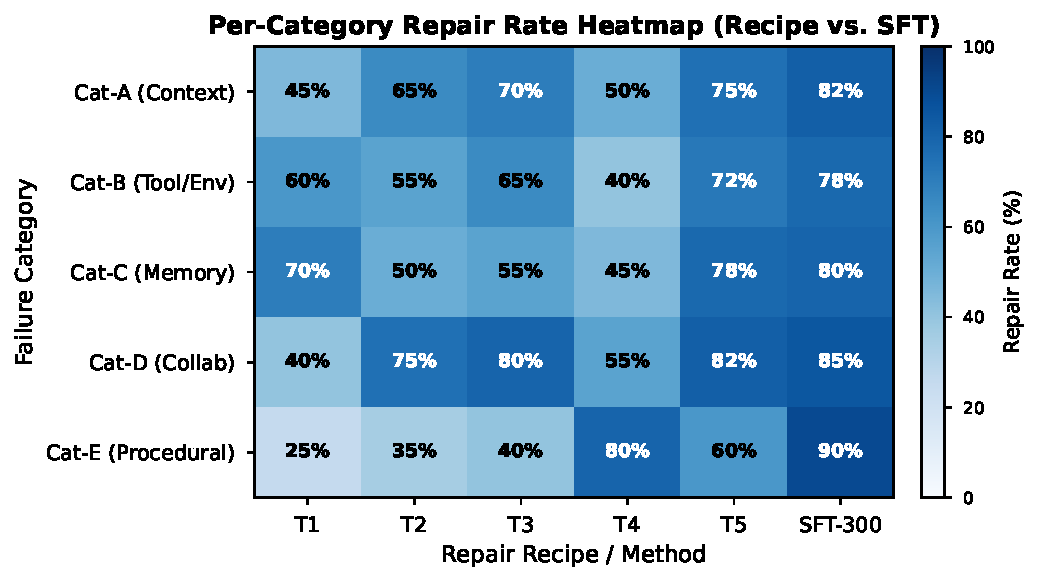
\includegraphics[width=\linewidth]{figs/category_repair_heatmap.pdf}
    \caption{Per-category repair rate heatmap for recipes T1--T5 and SFT-300 (mock data). Darker = higher repair rate. Cat.~E is hardest to repair without SFT.}
    \label{fig:repair-heatmap}
  \end{subfigure}
  \hfill
  \begin{subfigure}[b]{0.48\linewidth}
    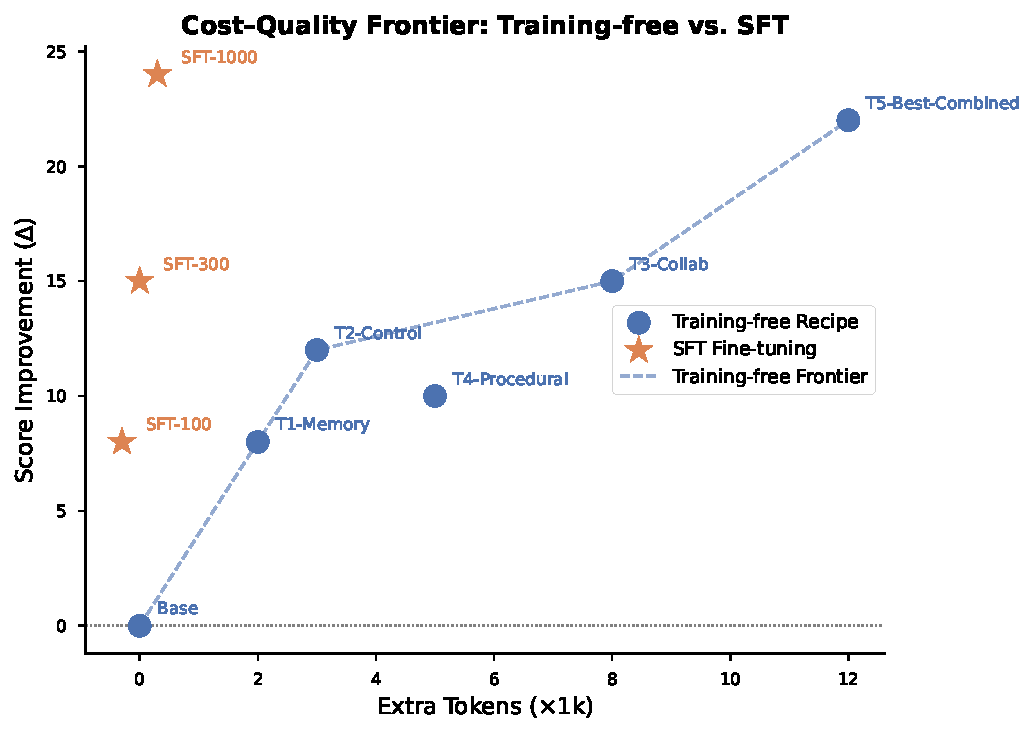
\includegraphics[width=\linewidth]{figs/cost_quality_frontier.pdf}
    \caption{Cost--quality frontier: extra tokens vs.\ score improvement $\Delta$. Training-free recipes (blue circles) vs.\ SFT variants (orange stars).}
    \label{fig:cost-quality}
  \end{subfigure}
  \caption{Repair analysis (mock data; to be replaced with real evaluation results). Left: per-category repair rates show T1--T3 are strongest on Cat.~C and Cat.~D; Right: SFT achieves higher $\Delta$ at zero token overhead but requires training.}
  \label{fig:repair-analysis}
\end{figure}
